\begin{figure}[!h]
\centering
\caption{Density gradient is robust to adding region and state fixed-effects}
\label{fig:big_CZ}
\subfloat[Raw wages]{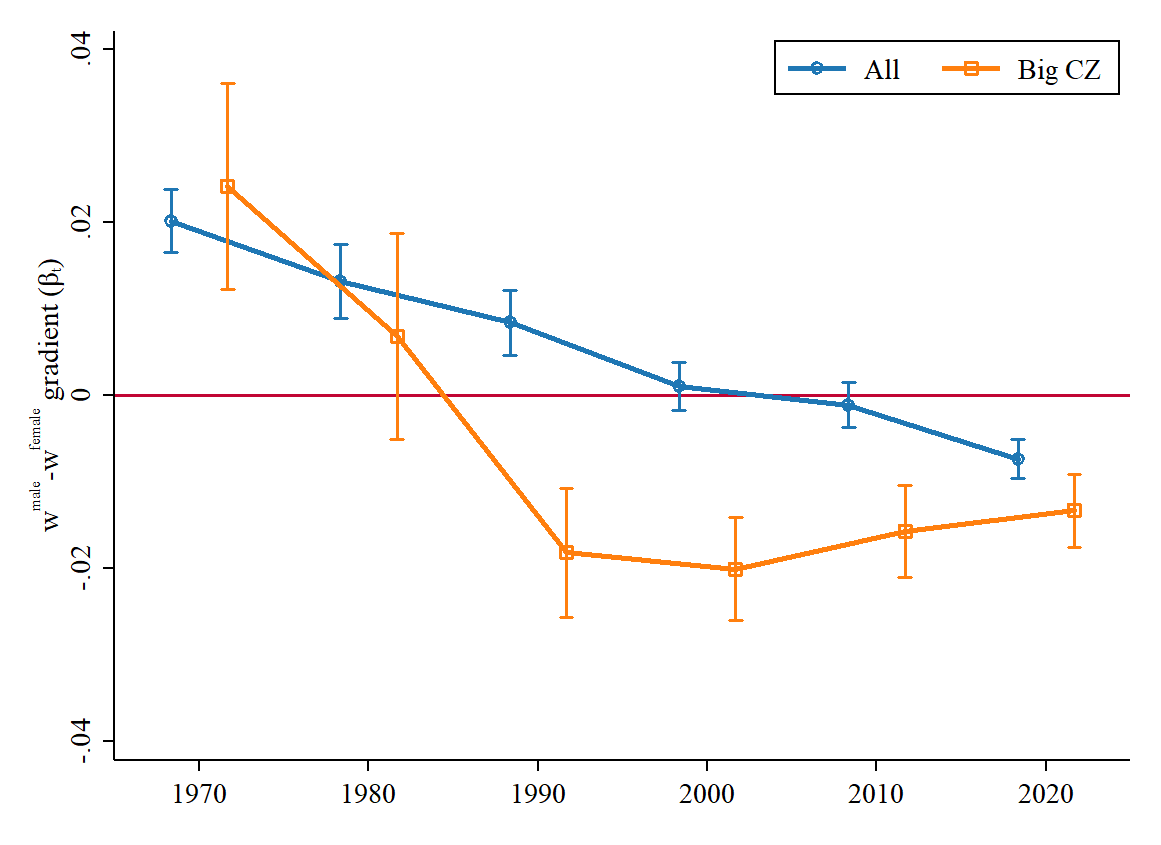
\includegraphics[width=.5\textwidth]{../2_analysis/output/figures/baseline_big_full_time}} \subfloat[Net of age/race]{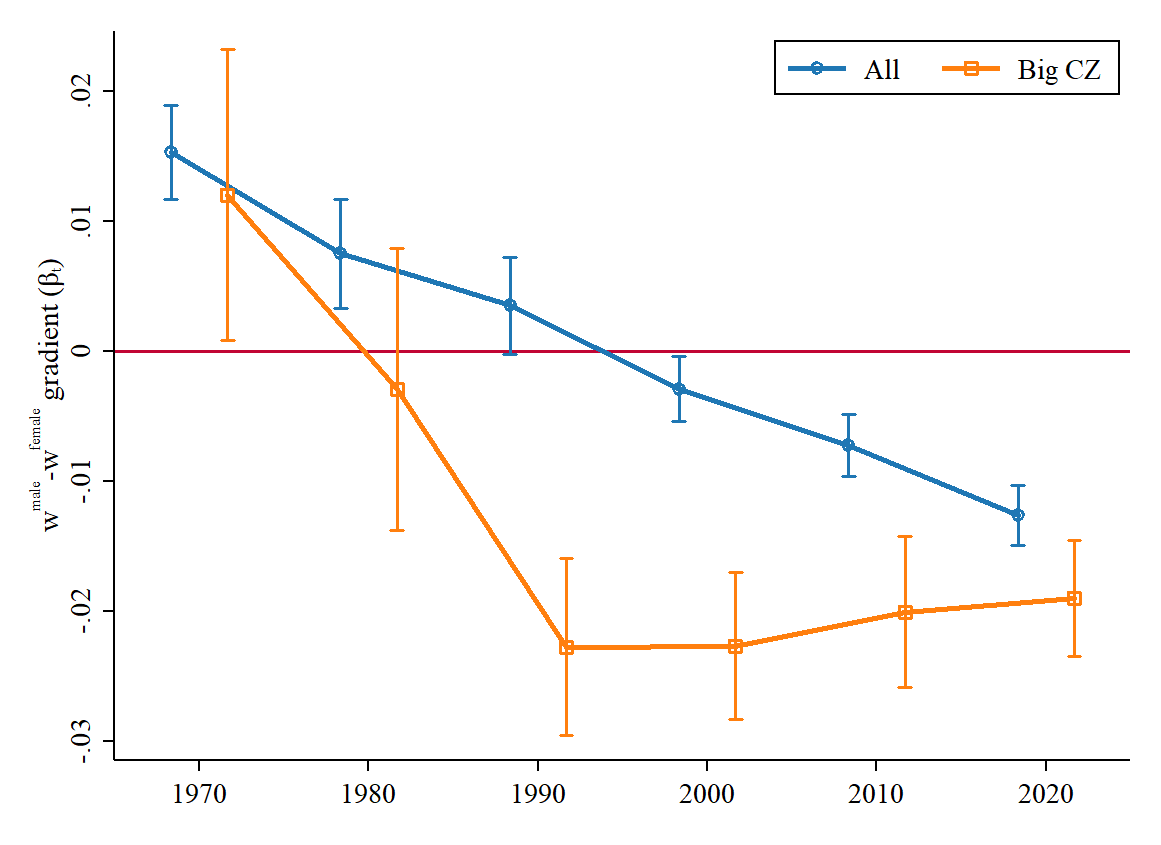
\includegraphics[width=.5\textwidth]{../2_analysis/output/figures/basic_big_full_time}} \\ 
\par \begin{minipage}[h]{\textwidth}{\tiny\textbf{Note:} figure restricts to CZ with more than 1 people per km$^2$. Bars show 90\% confidence intervals. Big CZ are defined as those having a density of at least 2 people per square km in 1950. Standard errors clustered at the CZ level. Figure generated on 23 Nov 2020 at 16:25:27. Figure generated using the dofile 2\_analysis/code\_files/write\_regression\_coefplots.do.}\end{minipage}
\end{figure}
